\documentclass[border=15pt, tikz]{standalone}
\usepackage[T1]{fontenc}
\usepackage[utf8]{inputenc}
\usepackage{tikz}
\usetikzlibrary{positioning, arrows.meta, decorations.pathreplacing, calc, fit}
\definecolor{clrattention}{HTML}{00B4D8}
\definecolor{clrattention_alt}{HTML}{90E0EF}
\definecolor{clrffn}{HTML}{E63946}
\definecolor{clrnorm}{HTML}{FFBE0B}
\definecolor{clrembed}{HTML}{06D6A0}
\definecolor{clrresidual}{HTML}{118AB2}
\definecolor{clroutput}{HTML}{7B2CBF}
\definecolor{clrspectral}{HTML}{00F5D4}
\definecolor{clrphysics}{HTML}{F77F00}
\definecolor{clrborder}{HTML}{073B4C}
\definecolor{clrtext}{HTML}{073B4C}
\definecolor{clrgroup_frame}{HTML}{073B4C}
\definecolor{clrgroup_fill}{HTML}{EDF6F9}
\begin{document}
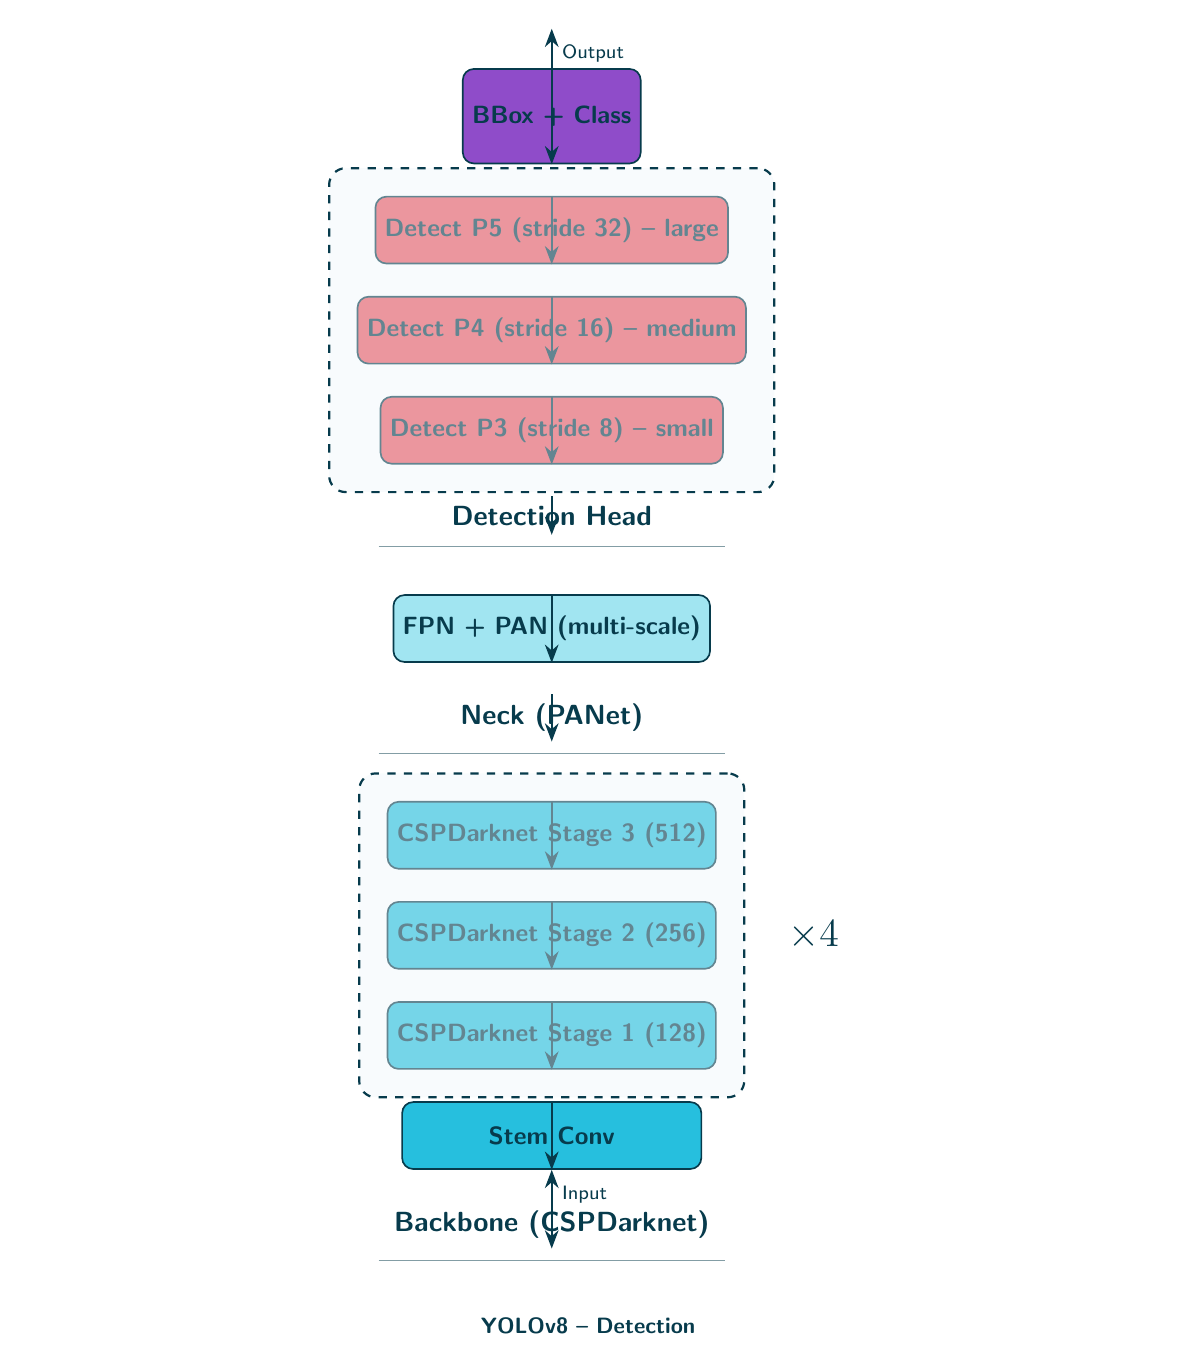
\begin{tikzpicture}[
    >=Stealth,
    every node/.style={font=\sffamily},
    block/.style={draw=clrborder, rounded corners=4pt, minimum width=3.8cm,
                  minimum height=0.85cm, font=\sffamily\small\bfseries,
                  text=clrtext, line width=0.6pt},
    arrow/.style={->, thick, color=clrborder, line width=0.8pt},
    skiparrow/.style={->, thick, color=clrresidual, line width=0.8pt, rounded corners=3pt},
    label/.style={font=\sffamily\scriptsize, text=clrtext},
    subtitle/.style={font=\sffamily\footnotesize, text=clrtext},
]
\node[inner sep=0, minimum height=0] (n_1_rule) at (0,0) {};
\draw[color=clrgroup_frame!50, line width=0.4pt] ([xshift=-2.2cm]n_1_rule.center) -- ([xshift=2.2cm]n_1_rule.center);
\node[above=4pt of n_1_rule, font=\sffamily\normalsize\bfseries, text=clrborder] (n_1) {Backbone (CSPDarknet)};
\node[block, fill=clrattention!85, minimum width=3.8cm, minimum height=0.85cm, text=clrtext, above=0.4cm of n_1] (n_2) {Stem Conv};
\node[block, fill=clrattention!85, minimum width=3.8cm, minimum height=0.85cm, text=clrtext, above=0.4cm of n_2] (n_3) {CSPDarknet Stage 1 (128)};
\node[block, fill=clrattention!85, minimum width=3.8cm, minimum height=0.85cm, text=clrtext, above=0.4cm of n_3] (n_4) {CSPDarknet Stage 2 (256)};
\node[block, fill=clrattention!85, minimum width=3.8cm, minimum height=0.85cm, text=clrtext, above=0.4cm of n_4] (n_5) {CSPDarknet Stage 3 (512)};
\node[above=0.6cm of n_5, inner sep=0, minimum height=0] (n_6_rule) {};
\draw[color=clrgroup_frame!50, line width=0.4pt] ([xshift=-2.2cm]n_6_rule.center) -- ([xshift=2.2cm]n_6_rule.center);
\node[above=4pt of n_6_rule, font=\sffamily\normalsize\bfseries, text=clrborder] (n_6) {Neck (PANet)};
\node[block, fill=clrattention_alt!85, minimum width=3.8cm, minimum height=0.85cm, text=clrtext, above=0.4cm of n_6] (n_7) {FPN + PAN (multi-scale)};
\node[above=0.6cm of n_7, inner sep=0, minimum height=0] (n_8_rule) {};
\draw[color=clrgroup_frame!50, line width=0.4pt] ([xshift=-2.2cm]n_8_rule.center) -- ([xshift=2.2cm]n_8_rule.center);
\node[above=4pt of n_8_rule, font=\sffamily\normalsize\bfseries, text=clrborder] (n_8) {Detection Head};
\node[block, fill=clrffn!85, minimum width=3.8cm, minimum height=0.85cm, text=clrtext, above=0.4cm of n_8] (n_9) {Detect P3 (stride 8) -- small};
\node[block, fill=clrffn!85, minimum width=3.8cm, minimum height=0.85cm, text=clrtext, above=0.4cm of n_9] (n_10) {Detect P4 (stride 16) -- medium};
\node[block, fill=clrffn!85, minimum width=3.8cm, minimum height=0.85cm, text=clrtext, above=0.4cm of n_10] (n_11) {Detect P5 (stride 32) -- large};
\node[block, fill=clroutput!85, minimum width=2.0cm, minimum height=1.2cm, text=clrtext, above=0.4cm of n_11] (n_12) {BBox + Class};
\draw[arrow] (n_1.north) -- (n_1.south);
\draw[arrow] (n_2.north) -- (n_2.south);
\draw[arrow] (n_3.north) -- (n_3.south);
\draw[arrow] (n_4.north) -- (n_4.south);
\draw[arrow] (n_5.north) -- (n_5.south);
\draw[arrow] (n_6.north) -- (n_6.south);
\draw[arrow] (n_7.north) -- (n_7.south);
\draw[arrow] (n_8.north) -- (n_8.south);
\draw[arrow] (n_9.north) -- (n_9.south);
\draw[arrow] (n_10.north) -- (n_10.south);
\draw[arrow] (n_11.north) -- (n_11.south);
\draw[arrow] (n_12.north) -- (n_12.south);
\draw[arrow] (n_2.south) ++ (0,-0.5) -- node[right, yshift=-2pt, font=\sffamily\scriptsize, text=clrtext] {Input} (n_2.south);
\draw[arrow] (n_12.north) -- node[right, yshift=-2pt, font=\sffamily\scriptsize, text=clrtext] {Output} ++ (0,0.5);
\node[draw=clrgroup_frame, rounded corners=6pt, dashed, line width=0.8pt, fill=clrgroup_fill, fill opacity=0.4, inner sep=0.35cm, fit=(n_3) (n_4) (n_5)] (g_0) {};
\node[right=12pt of g_0.east, anchor=west, font=\sffamily\Large\bfseries, text=clrborder] (g_0_badge) {$\times4$};
\node[draw=clrgroup_frame, rounded corners=6pt, dashed, line width=0.8pt, fill=clrgroup_fill, fill opacity=0.4, inner sep=0.35cm, fit=(n_9) (n_10) (n_11)] (g_1) {};
\node[below=0.6cm of current bounding box.south, subtitle, text width=14cm, align=center] {\textbf{YOLOv8 -- Detection}};
\end{tikzpicture}
\end{document}
